\chapter{Introduction}

\section{Recommended Reading}
Books to aide with the course, you are not expected to read them completely however you may find them useful to address topics from the slides.
\\ \\ \twosplit{
    \begin{center}
        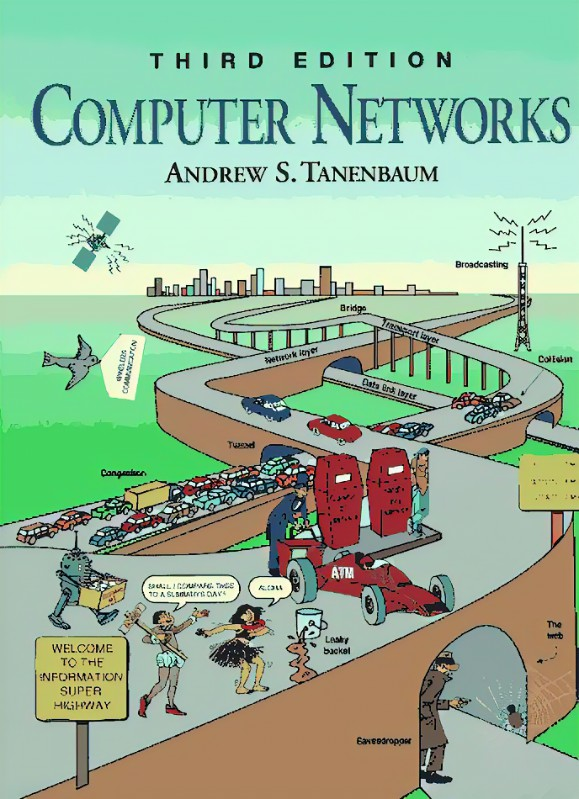
\includegraphics[height=6cm]{introduction/images/computer_networks_cover.jpeg}
        \\ \textbf{Computer Networks}
        \\ \textit{Andrew S. Tanenbaum}
        \\ \textit{5th or 4th edition suffice}
    \end{center}
}{
    \begin{center}
        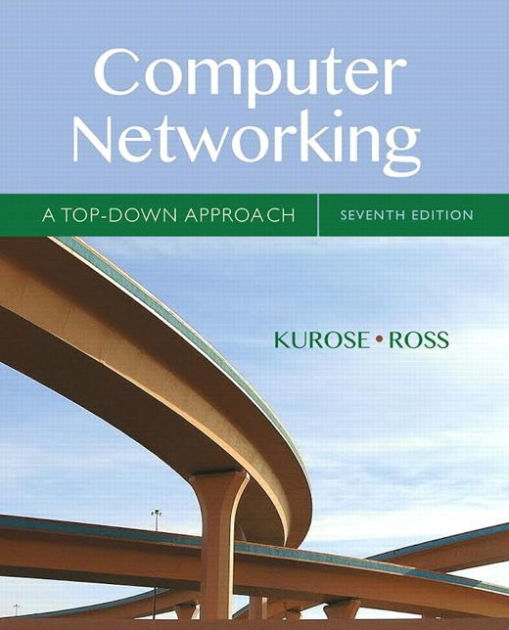
\includegraphics[height=6cm]{introduction/images/top_down_cover.jpeg}
        \\ \textbf{Computer Networking: A Top-Down Approach}
        \\ \textit{James Kurose and Keith Ross}
        \\ \textit{7th or 6th edition suffice, available from Imperial College Library}
    \end{center}
}

\section{What is Computer Networking?}
\begin{definitionbox}{Computer Networking}
    The process of interconnecting computer systems via telecommunications methods to share data and resources.
\end{definitionbox}

\begin{itemize}
    \setlength\itemsep{0em}
    \item Networks are becoming pervasive (everywhere, always on).
    \item Most mainstream software systems are distributed (cloud computing).
    \item Peformance often depends on network usage (can be a bottleneck or on critical path).
\end{itemize}

\begin{sidenotebox}{First Internet Connection}
    Arpanet (first part of the internet) was created on september 1st 1969 with a single node.
    \\
    \\ First message as "login", after "lo" was transmitted it crashed, but sent the result after rebooting an hour later.
    \\
    \\ Greatly expanded afterwords, connecting several universities.
    \begin{center}
        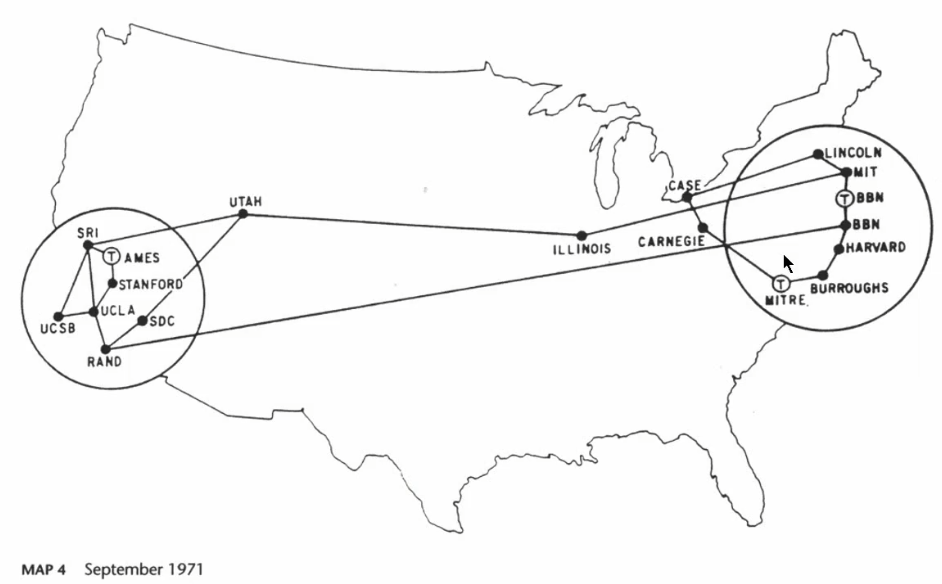
\includegraphics[width=\textwidth]{introduction/images/arpanet_sept_1971.png}
    \end{center}
\end{sidenotebox}

\begin{sidenotebox}{Vocations}
    \begin{tabular}{l p{.8\textwidth}}
        \textbf{Network Engineer/Architect}         & Design, build and maintain networks.                     \\
        \textbf{Server Application Developer}       & Server Backend and communication for cloud applications. \\
        \textbf{Network Software Engineer}          & Networks + Software Engineering                          \\
        \textbf{Data Center / Cloud Platform Admin} & Networks + Cloud Computing                               \\
        \textbf{Network Security Engineer}          & Networks + Computer Security                             \\
    \end{tabular}
\end{sidenotebox}
